\chapter{Branch and Bound}
In this chapter we analyze the first technique studied, the \textit{Branch and Bound}, based on the discarding of subset of solution candidates that are a priori known to be non-optimal. This can be achived by means of the estimation of lower bounds on the cost of the optimal solution.

\section{Heuristics for Lower Bounds}
\subsection{1-tree}
The first heuristic for computing a lower bound is the one based on a \textit{1-tree}. A 1-tree is a subgraph obtained from an another graph by removing a node, and all the edges connected to it. We can compute the \textit{minimum spanning tree} (\textsc{mst}) of the residual subgraph, and then connect the remaining node inserting its two lowest-cost edges in the \textsc{mst}, in order to have $|V|$ edges, which is the number of edges in an hamiltonian cycle in a graph. The \textsc{mst} can be computed in quadratic time with the Prim-Dijkstra algorithm.

In figure \ref{fig:1trees} two examples of 1-trees in complete graphs of various size: red edges are the ones in the 1-tree, while grey ones are the edges left out.

\begin{figure}[hbtp]
  \centering
  \subfloat[][\emph{Graph with 20 nodes}.]
  {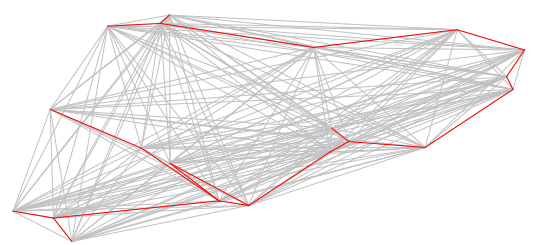
\includegraphics[width=.48\columnwidth]{images/1tree20.png}} \quad
  \subfloat[][\emph{Graph with 100 nodes}.]
  {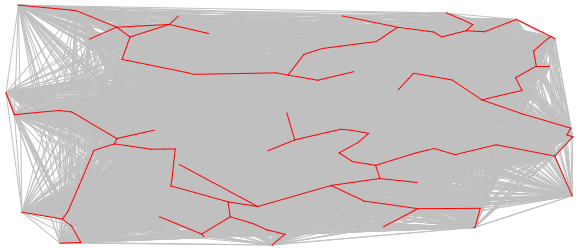
\includegraphics[width=.48\columnwidth]{images/1tree100.png}}
  \caption{Two examples of 1-trees computed from complete graphs.}
  \label{fig:1trees}
\end{figure}

Supposing node $1$ is the node left out from the \textsc{mst}, %
and $T$ is the optimal tour in $G$, then $T \cap \delta(1)$ are the two min-cost edges $\in \delta(1)$ 
and $T\: \backslash\: \delta(1)$ are the $|V|-2$ edges without cycles in the optimal tour, then
$$\cost(\mbox{the two min-cost edges} \in \delta(1)) \leq \cost(T \cap \delta(1))$$
$$\cost(\mbox{\textsc{mst}} \in G\: \backslash\: \delta(1)) \leq \cost(T \backslash \delta(1))$$
and therefore
$$\cost(\mbox{\textsc{mst}}+\mbox{the two min-cost edges} \in \delta(1)) \leq \cost(T),$$
this making the 1-tree a reasonable choice for a heuristic for a lower bound on the cost of the optimal tour in $G$.
